\section{Results}
\label{sec:results}

\subsection{RQ1: Static--Dynamic Fusion}

\subsubsection{Overall comparison}

Table~\ref{tab:fusion-main} reports the fusion-only comparison on all 1,922
paired samples. Average produces the highest AUC among the simple nonadaptive
rules (0.9840) and the lowest Brier score overall (0.0450). This strong baseline
prevents the adaptive family from being judged only against a weak fixed rule.
Max-risk performs worst in ranking, FPR, and Brier, showing that always taking
the larger risk score amplifies channel errors.

\begin{table*}[t]
\centering
\caption{Fusion comparison on 1,922 paired MalBehavD-V1 samples. Adaptive
P/PI/PID are measured development evidence on the same cohort used during method
development. FPR and TPR are reported together at validation-selected operating
points.}
\label{tab:fusion-main}
\small
\begin{tabular}{lccccc}
\toprule
Method & ROC--AUC & AP & FPR (\%) & TPR (\%) & Brier \\
\midrule
Average 50/50 & \textbf{0.9840} & 0.9880 & 14.70 & \textbf{96.77} & \textbf{0.0450} \\
Max-risk & 0.9779 & 0.9794 & 16.63 & \textbf{96.77} & 0.0604 \\
Fixed weight & 0.9821 & 0.9862 & 12.45 & 96.06 & 0.0487 \\
Logistic stacking & 0.9819 & 0.9867 & 14.91 & 96.57 & 0.0454 \\
Adaptive P & 0.9827 & 0.9867 & \textbf{11.16} & 95.96 & 0.0456 \\
Adaptive PI & 0.9827 & 0.9867 & 11.48 & 95.96 & 0.0456 \\
Full PID & 0.9828 & \textbf{0.9868} & 11.59 & 95.96 & 0.0455 \\
\bottomrule
\end{tabular}
\end{table*}

Adaptive P attains the lowest observed FPR, 11.16\%, while preserving TPR close
to Fixed (95.96\% versus 96.06\%). PI and PID provide nearly identical AUC/AP and
TPR and slightly higher FPR than P. Full PID is therefore not the best member of
its own nested family for the selected operating-point objective. The result
supports present-disagreement adaptation, not a generic advantage for all three
controller terms.

Figure~\ref{fig:fusion-summary} displays the metric trade-off. Average leads AUC
and Brier by small margins; Adaptive P leads FPR. Ranking and operating-point
objectives select different methods. This is why the paper does not collapse the
evaluation into one “best fusion” statement.

\begin{figure*}[t]
\centering
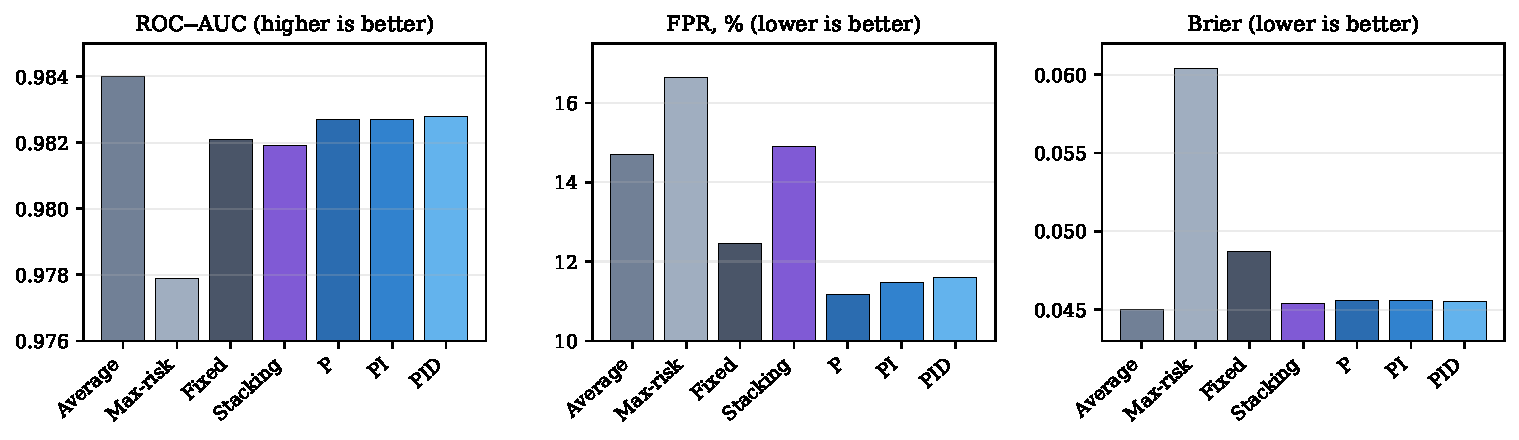
\includegraphics[width=0.94\textwidth]{fusion_summary.pdf}
\caption{Fusion discrimination, false-positive rate, and Brier score on the
paired development cohort. Values are aggregate means supplied by the retained
report; error bars are omitted because method-level fold vectors are not present
in this writing checkout.}
\label{fig:fusion-summary}
\end{figure*}

\subsubsection{Paired effects and controller ablation}

Table~\ref{tab:fusion-effects} reports the paired comparisons that govern the
claim. Adaptive P reduces FPR by 1.28 percentage points relative to Fixed, with
95\% CI $[-2.47,-0.11]$. It also reduces Brier by 0.00306, with CI
$[-0.00585,-0.00030]$. The TPR difference is $-0.10$ percentage point and its
interval crosses zero. In counts, P produces 104 false positives versus 116 for
Fixed and 950 true positives versus 951. The supported statement is improved FPR
and calibration with no detected material TPR loss on this development cohort.

\begin{table*}[t]
\centering
\caption{Primary paired fusion effects. Percentage-point (pp) effects are method
minus comparator. The two methods in a row can use independently validation-
selected thresholds.}
\label{tab:fusion-effects}
\small
\setlength{\tabcolsep}{3.5pt}
\begin{tabular}{p{3.1cm}p{2.6cm}p{2.1cm}p{3.0cm}p{4.0cm}}
\toprule
Comparison & Metric & Difference & 95\% CI & Interpretation \\
\midrule
Adaptive P $-$ Fixed & FPR & $-1.28$ pp & $[-2.47,-0.11]$ & Lower observed false-positive rate \\
Adaptive P $-$ Fixed & Brier & $-0.00306$ & $[-0.00585,-0.00030]$ & Lower squared probability error \\
Adaptive P $-$ Fixed & TPR & $-0.10$ pp & includes 0 & No detected TPR difference \\
Full PID $-$ Stacking & FPR & $-3.32$ pp & $[-4.94,-1.72]$ & Lower FPR at separately selected operating point \\
Full PID $-$ Stacking & AUC & $+0.08$ pp & $[-0.19,+0.37]$ & Comparable ranking; interval includes 0 \\
Full PID $-$ Stacking & TPR & $-0.62$ pp & $[-1.21,0.00]$ & Small sensitivity trade-off \\
Full PID $-$ Adaptive P & FPR & $+0.43$ pp & $[+0.11,+0.86]$ & I/D worsen FPR relative to P \\
\bottomrule
\end{tabular}
\end{table*}

Full PID versus Logistic stacking illustrates a different trade-off. PID lowers
FPR by 3.32 percentage points, but the thresholds are selected independently and
TPR is 0.62 percentage point lower. Its AUC difference is only $+0.08$
percentage point with an interval spanning zero. We therefore describe AUC as
comparable and avoid a same-TPR or universal-superiority claim.

The nested comparison is decisive for controller complexity. Full PID increases
FPR by 0.43 percentage point over Adaptive P while TPR is unchanged. The original
confirmatory ablation reached the same qualitative conclusion: turning off
$K_d$ while retaining $K_p,K_i$ changed none of the 1,922 final decisions, and D
altered only 6 of 7,688 intermediate-prefix decisions before the differences
disappeared at the final prefix. PID minus PI AUC was $-0.000125$ with an
interval crossing zero. Thus the retained event horizon does not support a
derivative benefit, and the integral term also fails to improve on P.

\subsubsection{Answer to RQ1}

Current static--dynamic disagreement can usefully adapt the mixture: Adaptive P
improves FPR and Brier over Fixed on the measured development cohort. Full PID
can achieve AUC comparable to learned stacking and a lower FPR at its own
selected operating point, with a small TPR trade-off. The available evidence
does not support incremental I/D complexity, closed-loop stability, sleep-
evasion handling, wall-clock latency reduction, or external validation.

\subsection{RQ2: Explanation-Guided Label Allocation}

\subsubsection{Learning-curve quality and target attainment}

Table~\ref{tab:al-main} integrates performance across 200--1,200 training labels.
$U+H$ achieves the highest ROC-AULC (0.933026) and AP-AULC (0.883336). Relative
to Random, its paired fold improvements are +0.004249 ROC-AULC and +0.014985
AP-AULC in the favorable direction in all five folds. Gains over Uncertainty are
smaller: +0.001754 and +0.001401, favorable in four of five folds.

\begin{table*}[t]
\centering
\caption{Confirmatory active-learning performance, target attainment, and
computation. Labels-to-target excludes validation labels and full-pool reference
cost.}
\label{tab:al-main}
\small
\setlength{\tabcolsep}{5pt}
\begin{tabular}{lccccc}
\toprule
Policy & ROC-AULC & AP-AULC & Labels to target & Query, 10 rounds (s) & Model + query (s) \\
\midrule
Random & 0.928777 & 0.868350 & 584 & 0.0194 & 4.1947 \\
Uncertainty & 0.931272 & 0.881934 & 520 & 0.0191 & 4.1454 \\
$U+H$ & \textbf{0.933026} & \textbf{0.883336} & 508 & 0.2459 & 4.4741 \\
$U+V$ & 0.930377 & 0.880164 & \textbf{488} & 0.2298 & 4.3826 \\
\xfull & 0.932202 & 0.881638 & 492 & 0.2358 & 4.3471 \\
\bottomrule
\end{tabular}
\end{table*}

$U+V$ reaches the validation target with the fewest mean training labels (488),
while \xfull reaches it with 492. Relative to Random's 584, \xfull reduces
the mean training budget by 92 labels, or 15.8\%. It also uses 28 fewer labels
than Uncertainty, but this advantage does not imply consistent superiority in
learning-curve ranking. Figure~\ref{fig:al-summary} shows that each
explanation-guided policy emphasizes a different criterion.

\begin{figure*}[t]
\centering
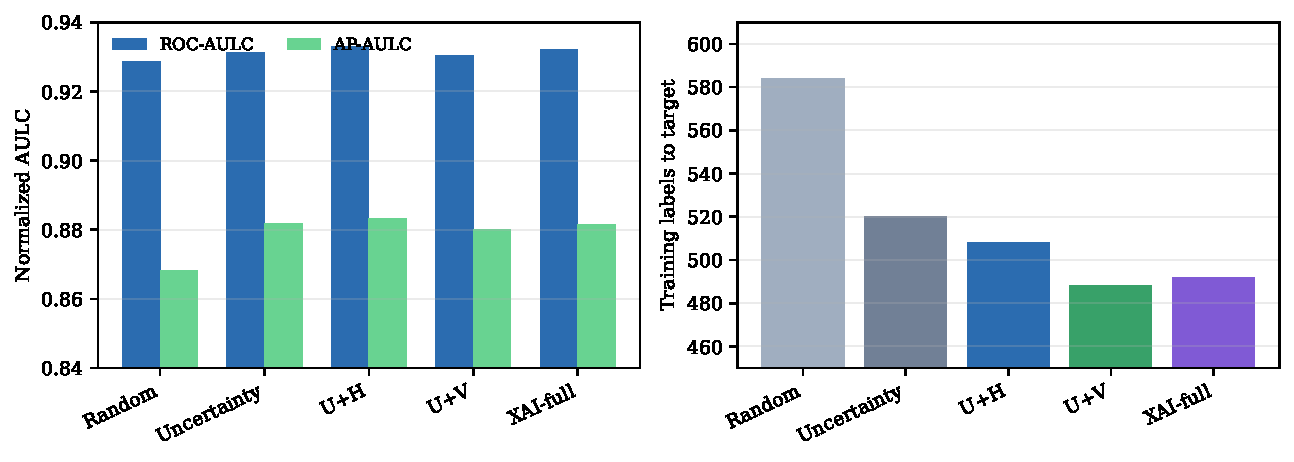
\includegraphics[width=0.93\textwidth]{al_summary.pdf}
\caption{Confirmatory active-learning summaries. Higher AULC is better; fewer
training labels to the predeclared validation target are better. Error bars are
omitted because the source-of-truth report provides aggregate means and paired
effects rather than fold vectors in this checkout.}
\label{fig:al-summary}
\end{figure*}

\begin{table}[t]
\centering
\caption{Selected paired outer-fold AL effects.}
\label{tab:al-effects}
\scriptsize
\setlength{\tabcolsep}{1pt}
\begin{tabular}{@{}lrrc@{}}
\toprule
Comparison & $\Delta$ROC & $\Delta$AP & Favorable folds \\
\midrule
$U+H$ vs. Random & +0.004249 & +0.014985 & 5/5 \\
$U+H$ vs. Uncertainty & +0.001754 & +0.001401 & 4/5 \\
\xfull vs. Random & +0.003425 & +0.013287 & 5/5 \\
\xfull vs. Uncertainty & +0.000931 & $-0.000297$ & 3/5 ROC \\
\bottomrule
\end{tabular}
\end{table}

Table~\ref{tab:al-effects} limits the strongest claim. \xfull improves over
Random in both AULC metrics and all five fold directions, but its AP-AULC
difference from Uncertainty is slightly negative and its ROC improvement occurs
in only three of five folds. Directional entropy provides the most consistent
measured addition; the three-signal policy is not a universal winner.

\subsubsection{Restricted-FPR behavior and computation}

Table~\ref{tab:low-fpr} shows that Uncertainty remains strong in restricted-FPR
regions. It leads normalized partial AUC at FPR$\leq5\%$ and TPR-AULC at the 1\%
cap; \xfull leads only at the 5\% cap. Explanation-guided policies clearly
improve over Random, but their differences from Uncertainty are small and metric
dependent. Each outer test fold contains roughly 300 benign rows, so a single
false positive changes FPR by about 0.33 percentage point. The data cannot
resolve production regions several orders of magnitude lower.

\begin{table*}[t]
\centering
\caption{Active-learning summaries in restricted false-positive regions.}
\label{tab:low-fpr}
\small
\begin{tabular}{lccc}
\toprule
Policy & pAUC, FPR$\leq5\%$ & TPR-AULC, FPR cap 1\% & TPR-AULC, FPR cap 5\% \\
\midrule
Random & 0.804096 & 0.580620 & 0.731980 \\
Uncertainty & \textbf{0.826300} & \textbf{0.638180} & 0.769260 \\
$U+H$ & 0.824774 & 0.636780 & 0.770620 \\
$U+V$ & 0.825194 & 0.626260 & 0.768140 \\
\xfull & 0.823525 & 0.631860 & \textbf{0.771460} \\
\bottomrule
\end{tabular}
\end{table*}

$U+H$ increases total model-plus-query time by about 7.93\% relative to
Uncertainty. \xfull increases it by 4.86\%, and query computation accounts
for approximately 5.42\% of its reported model-plus-query time. These small
absolute times apply to a 2,000-row experiment and omit analyst annotation and
production feature extraction.

\subsubsection{Answer to RQ2}

Explanation-derived signals add useful information relative to random
acquisition. Directional entropy yields the strongest integrated learning
trajectory; variance reaches the declared target with the fewest labels; and the
full policy saves 92 training labels relative to Random. Improvements over
uncertainty alone are smaller and change with the metric. The evidence supports
objective-dependent sample prioritization, not a single dominant policy or a
measured reduction in analyst hours.

\subsection{RQ3: Quantitative TreeSHAP Validation}

\subsubsection{Controlled deletion}

Table~\ref{tab:deletion} reports AUC decreases over 25 fitted models. Top-
$|\mathrm{SHAP}|$ deletion has a large monotonic effect as $k$ increases, whereas
uniform random deletion remains near zero. Under mean replacement at $k=50$,
the decreases are 0.306729 and 0.000979, an absolute difference of 0.305750.
Median replacement gives a similar difference of 0.300119. The conclusion is
robust to the two training-derived replacement baselines.

\begin{table*}[t]
\centering
\caption{Controlled feature-space deletion. Values are ROC--AUC decreases from
the corresponding unmasked model.}
\label{tab:deletion}
\small
\begin{tabular}{lrrrr}
\toprule
Replacement & $k$ & Top-SHAP drop & Random drop & Top minus random \\
\midrule
Mean & 10 & 0.047817 & 0.000200 & 0.047617 \\
Mean & 25 & 0.135853 & 0.000530 & 0.135323 \\
Mean & 50 & \textbf{0.306729} & 0.000979 & \textbf{0.305750} \\
Median & 10 & 0.053483 & 0.000094 & 0.053388 \\
Median & 25 & 0.125180 & 0.000326 & 0.124854 \\
Median & 50 & \textbf{0.300777} & 0.000658 & \textbf{0.300119} \\
\bottomrule
\end{tabular}
\end{table*}

\begin{figure}[t]
\centering
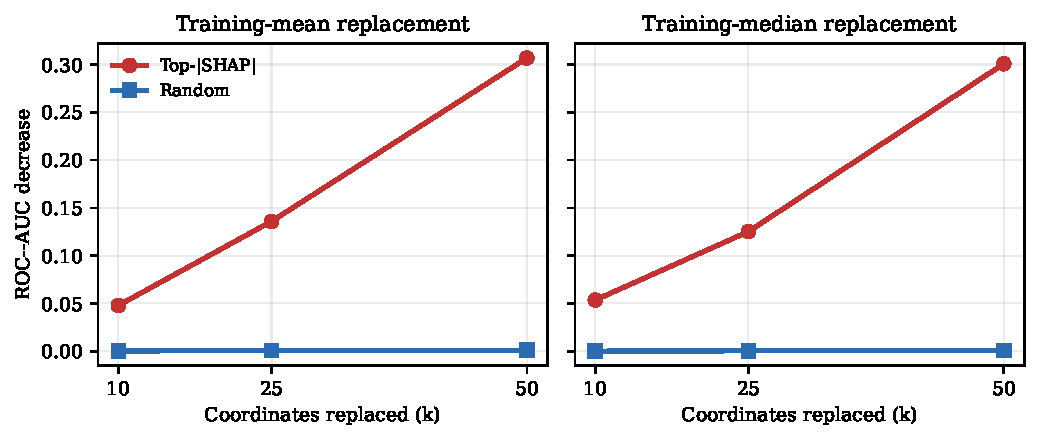
\includegraphics[width=\linewidth]{fidelity_deletion_confirmatory.pdf}
\caption{AUC decrease under top-$|\mathrm{SHAP}|$ and equal-count random
replacement. Absolute effects are emphasized because a ratio is unstable when
the random-control decrease is near zero.}
\label{fig:deletion}
\end{figure}

Equal coordinate count is an incomplete control. Uniform masks often select
inactive tree features and do not match standardized displacement or manifold
distance. The result nevertheless demonstrates relative fitted-model reliance:
under both specified interventions, TreeSHAP ranks coordinates whose replacement
changes ranking much more than uniformly chosen coordinates. It does not show a
valid edit to a PE file or a causal malware mechanism.

\subsubsection{Rank stability}

Within a fixed fold, global Spearman agreement is 0.6144, and top-10 Jaccard
agreement is 0.6221. Across folds, Spearman falls to 0.5512 and top-10 Jaccard to
0.4416. Agreement decreases further at larger top sets across folds. The ranking
is therefore neither arbitrary nor invariant; the training partition changes it
more than controlled model randomness.

\begin{table}[t]
\centering
\caption{TreeSHAP ranking stability.}
\label{tab:stability}
\scriptsize
\begin{tabular}{lrrrr}
\toprule
Comparison & $\rho$ & $J_{10}$ & $J_{25}$ & $J_{50}$ \\
\midrule
Seed, same fold & 0.6144 & 0.6221 & 0.5398 & 0.4901 \\
Different fold & 0.5512 & 0.4416 & 0.3073 & 0.3020 \\
\bottomrule
\end{tabular}
\end{table}

\begin{figure}[t]
\centering
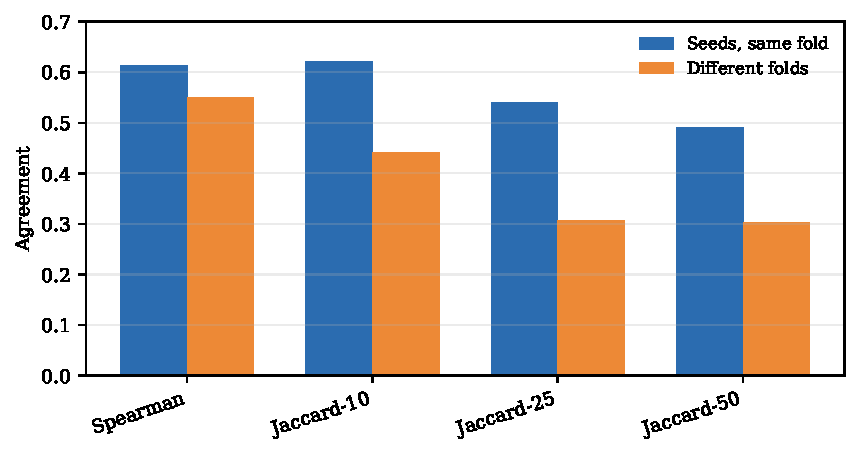
\includegraphics[width=\linewidth]{shap_stability_confirmatory.pdf}
\caption{Global and top-$k$ attribution agreement. Fold changes have a larger
effect than seed changes within the same fold.}
\label{fig:stability}
\end{figure}

Mean EC is $0.4268\pm0.0363$ and mean CF is $0.4680\pm0.0465$ across 25 models.
Maximum additivity error is approximately $6\times10^{-15}$. These values
describe geometry and numerical consistency; they are not combined into a
fidelity certificate.

\subsubsection{Answer to RQ3}

TreeSHAP top-ranked coordinates exert substantially greater model-ranking impact
than equal-budget random coordinates under both mean and median replacement.
Moderate stability supports repeatable model reliance while exposing meaningful
partition sensitivity. The evidence is quantitative but model relative: it does
not establish feature causality, executable-valid masking, or timeless malware
semantics.

\subsection{Exploratory Fusion Extensions}

The 1,186-sample horizon-40 subset was used after observing the horizon-20
limitations and is therefore exploratory. Robust PID v2 reached AUC 0.9895 and
AP 0.9911, equal at reported precision to Logistic stacking, with FPR 3.35\%
versus 3.68\% and TPR 94.32\% versus 94.84\%. The AUC difference interval
$[-0.0008,+0.0008]$ and FPR interval both include zero. Against the older PID
full v2, Robust PID v2 reduces FPR by 1.33 percentage points with CI
$[-2.66,-0.15]$. This supports an algorithm candidate, not independent
confirmation.

A gated residual PID stress test under a controlled five-event delay reports FPR
2.61\% versus 3.93\% for Temporal stacking and TPR 94.49\% versus 94.66\%.
It removes eight false positives, creates none, and loses one true positive;
Holm-adjusted $p=0.0312$. Three of five folds select zero gain, and event-AULC
does not improve. This evidence is limited to the specified stress construction.

Finally, the timestamp pilot downloads reports for 20 selected samples and finds
eight usable event sequences with 4,697 API--timestamp pairs. It demonstrates
that wall-clock sequences can be parsed. With only two usable benign and six
malware sequences, it cannot evaluate performance, latency, or the derivative
term. These exploratory results define the next confirmatory experiment and do
not change the main RQ1 conclusion.
